\chapter{Anexo III - Manuales de usuario e Instalación}

En este anexo se incluirán todos los manuales de usuario e instalación sobre aquellas herramientas que se crean necesarias para el desarrollo y comprobación de funcionamiento del \gls{tfg}. De forma adicional, se comentará cómo funcionan los scripts de instalación generados para que cualquier persona interesada en replicar los distintos casos de uso, tenga un fácil acceso a ellos. 

\section{Instalación de dependencias de los casos de uso}
\label{deps}

La motivación de esta sección es plasmar en un punto como hacer uso de las herramientas que se han dejado desarrolladas para la instalación de las dependencias de los casos de uso. Como ya se indicó en el Pliego de condiciones, al tener dos entornos de trabajo muy diferenciados se iban a crear dos máquinas virtuales (\ref{maquina_p4}, \ref{maquina_xdp})  para conseguir aislar todo posible conflicto de dependencias. A continuación, se indicará como instalar las dependencias asociadas a cada entorno.

\subsection{Instalación de dependencias máquina \glsentryshort{xdp}}

La tecnología XDP, al ser desarrollada propiamente en el Kernel de Linux, no necesitará de muchas dependencias para trabajar con ella. Todas las dependencias inducidas vienen por la necesidad de ciertos compiladores para establecer todo el proceso de compilación de un programa \gls{xdp}, desde su C restringido hasta su forma de bytecode. Para instalar dichas dependencias se necesitará haber descargado el repositorio de este \gls{tfg} en local. Esto se puede realizar según se indica en el bloque \ref{code:xdp_deps}.

\begin{lstlisting}[language= bash, style=Consola, caption={Descarga del repositorio del TFG},label=code:xdp_deps]
    # En caso de no tener "git" instalado lo podemos hacer de la siguiente forma
    sudo apt install -y git
    
    
    # Una vez que está instalado git, haremos un "clone" del repositorio
    git clone https://github.com/davidcawork/TFG.git
\end{lstlisting}

\vspace{0.5cm}

Una vez descargado el repositorio se debería encontrar un directorio llamado \gls{tfg} en el directorio donde se haya ejecutado dicho comando. El siguiente paso para instalar las dependencias, será movernos hasta el directorio de los casos de uso \gls{xdp} y lanzar el script de instalación con permisos de super-usuario según se indica en el bloque \ref{code:xdp_deps2}.

\begin{lstlisting}[language= bash, style=Consola, caption={Instalación de dependencias XDP},label=code:xdp_deps2]
    # Nos movemos al directorio de los casos de uso XDP
    cd TFG/src/use_cases/xdp/
    
    # Lanzamos el script de instalación con permisos de super usuario
    sudo ./install.sh
\end{lstlisting}

\vspace{0.5cm}
Este script de instalación añadirá los siguientes paquetes e inicializará el submódulo de la librería \texttt{libbpf}:

\begin{itemize}
    \item Paquetes necesarios para el proceso de compilación de programas \gls{xdp}: \texttt{clang llvm libelf-dev gcc-multilib}
    \item Paquete necesario para tener todos los archivos de cabecera del Kernel que se tenga instalado:
    \texttt{linux-tools-\$(uname -r)}
    \item Paquete necesario en caso de querer hacer debug vía excepciones con la herramienta perf: \texttt{linux-tools-generic}
\end{itemize}

Por último, se quiere comentar el hecho de que es muy recomendable tener una versión superior a la \texttt{v4.12.0} de iproute2 ya que en versiones anteriores no se da soporte para \gls{xdp}. En Ubuntu 18.04 ya viene por defecto una versión compatible con \gls{xdp} por lo que no será necesario actualizarla, más información en el punto \ref{iproute2}.


\subsection{Instalación de dependencias máquina P4}

El entorno de trabajo P4 es bastante áspero y complicado, ya que se requieren de numerosas dependencias para poder empezar a trabajar con la tecnología P4. Por ello, para la instalación del entorno de P4 se ha dejado un script de instalación en el directorio de los casos de uso P4, bajo la carpeta \texttt{vm} con el nombre de \texttt{install.sh}. En el repositorio oficial, hay un método de instalación similar pero enfocado a un aprovisionamiento de Vagrant\footnote{\url{https://www.vagrantup.com/}}. \\
\par
El equipo de \textit{p4lang} monta una máquina virtual personalizada que al parecer del autor de este \gls{tfg} es demasiado \textit{User Friendly} ya que deja poco margen de maniobra para hacer una instalación más perfilada a un entorno de desarrollo real. Por ello, se ha tenido que desarrollar un script propio para su instalación. Esta nueva vía de instalación fue ofrecida en forma de pull-request al equipo \textit{p4lang} se puede consultar \href{https://github.com/p4lang/tutorials/pull/261}{\textbf{aquí}}.\\
\par

En primer lugar, se debe descargar el repositorio de este \gls{tfg}. Si no lo ha hecho aún puede consultarlo en el bloque \ref{code:xdp_deps}. Acto seguido, se deberá navegar hasta el directorio de los casos de uso P4 y lanzar el script como se indica en el bloque \ref{code:p4_deps}.

\begin{lstlisting}[language= bash, style=Consola, caption={Instalación de dependencias P4},label=code:p4_deps]
    # Nos movemos al directorio de los casos de uso XDP
    cd TFG/src/use_cases/p4/
    
    # Lanzamos el script de instalación con permisos de super usuario
    sudo ./vm/install.sh -q
\end{lstlisting}

Este script de instalación añadirá los siguientes paquetes y herramientas necesarias para el desarrollo en P4:

\begin{itemize}
    \item Paquetes necesarios que son dependencias de las herramientas principales de P4env. 
    \item Herramientas del P4env: \texttt{P4C PI P4Runtime}
    \item Paquetes necesarios para la prueba de P4: \texttt{Mininet BMV2 gRPC Protobuf}
\end{itemize}


%%%%%%%%%%%%%%%%%%%%%%%%%%%%%%%%%%%%%%%%%%%%%%%%%%%%%%%%%%%%%%%%%%%%%%%%%%%%%%%%%%%%%%%%%
\section{Herramienta \texttt{iproute2}}
\label{iproute2}
 Se ha querido añadir esta sección, ya que la herramienta iproute2 va a ser fundamental a la hora de cargar los programas \gls{xdp} en el Kernel, consultar interfaces, o verificar en que \textit{Network namespace} se encuentra el usuario. Por todo lo anterior, la herramienta iproute2 será una de las piezas claves para gestión de las \textit{Network Namespaces}, y la verificación de los casos de uso. 



\subsection{¿Qué es \texttt{iproute2?}}

Iproute2 es un paquete utilitario de herramientas para la gestión del \textit{Networking} en los sistemas Linux. Además, se encuentra ya en la mayoría de las distribuciones actuales. Sus desarrolladores principales son Alexey Kuznetsov y Stephen Hemminger, aunque hoy en día es un proyecto opensource donde cientos de personas contribuyen activamente en el repositorio\footnote{\url{https://github.com/shemminger/iproute2}}.  \\
\par
Actualmente, la versión más reciente de la herramienta es \texttt{v5.2.0}. Dicha versión será la que se utilizará en Ubuntu 18.04. El conjunto de utilidades que ofrece iproute2 está pensado para la sustitución de herramientas que se recogen en el paquete de \textbf{net-tools}, como por ejemplo a \texttt{ifconfig}, \texttt{route}, \texttt{netstat}, \texttt{arp}, etc. En la tabla \ref{tab:ipNettools} se pueden apreciar las herramientas de net-tools equivalentes en iproute2.

\begin{table}[ht]
\centering
\begin{tabular}{|c|c|}
\hline
\rowcolor[HTML]{C0C0C0} 
{\color[HTML]{000000} \textbf{net-tools}} & {\color[HTML]{000000} \textbf{iproute2}} \\ \hline
\texttt{arp}                                       & \texttt{ip neigh}                                 \\ \hline
\texttt{ifconfig}                                  & \texttt{ip link}                                  \\ \hline
\texttt{ifconfig -a}                               & \texttt{ip addr}                                  \\ \hline
\texttt{iptunnel}                                  & \texttt{ip tunnel}                                \\ \hline
\texttt{route}                                     & \texttt{ip route}                                 \\ \hline
\end{tabular}
\caption{Comparativa de herramientas Iproute2 con paquete net-tools}
\label{tab:ipNettools}
\end{table}

\subsection{¿Por qué necesitamos \texttt{iproute2}?}

Cuando se está trabajando con los programas XDP y se quiere comprobar su funcionamiento, se debe compilarlos. Esto se hará con los compiladores LLVM\footnote{\url{https://llvm.org/}} más clang\footnote{\url{https://clang.llvm.org/}}, como ya se comentaba en el estado del arte. Este proceso de compilación convertirá el código de los programas \gls{xdp}, en un \textit{bytecode} \gls{bpf}, y más tarde, se almacenará este \textit{bytecode} en un fichero de tipo \gls{elf}. Una vez compilados, se tendrá que anclarlos en el Kernel, y es  en este punto es donde entrará iproute2, ya que tiene un cargador \gls{elf} ( generalmente se trabajará con extensiones del tipo *.o ). \newline
\newline
Además, la herramienta iproute2 permite al usuario comprobar si una interfaz tiene cargado un programa \gls{xdp}. Arrojando en dicho caso, el identificador del programa \gls{xdp}, que tiene anclado la interfaz y si este programa está cargado de una forma nativa o de una forma genérica. Al final de la esta sección, se indicará cómo hacer esta comprobación.

\subsection{Estudio de compatibilidad de la herramienta \texttt{iproute2} en Ubuntu}

Al trabajar con esta herramienta para cargar programas XDP, se necesita  la versión que soporte el cargador ficheros \gls{elf}. Si usted tiene la versión de iproute2 que viene instalada por defecto en Ubuntu 16.04, le indicamos que aún no da soporte a \gls{xdp}. Inicialmente se buscó información relativa a partir de que versión se daba soporte a \gls{xdp} tanto en Ubuntu 16.04, como en Ubuntu 18.04. Como no se encontró información precisa sobre ello, se ha realizado un estudio de la compatibilidad de iproute2 a través de Ubuntu 16.04 y Ubuntu 18.04.\\ 
\par

Este estudio de compatibilidad se llevó a cabo descargando cada versión de iproute2, compilándola, e instalándola en nuestra máquina. Por último, para verificar si dicha versión daba soporte a \gls{xdp}, se comprobaba si un programa \gls{xdp} genérico que se sabía que funcionaba, cargaba o no, y si éste mostraba estadísticas sobre su carga. Más adelante, se indicará cómo compilar e instalar una versión en particular de iproute2.  \\ 
\par

Como se puede apreciar en la siguiente tabla \ref{tab:iproute}, en Ubuntu 16.04 a partir de la versión \texttt{v4.14.0} no existe compatibilidad. Esto es debido a que requiere librerías de enlazado extensible de formato (No \gls{elf} Support). Para resolver este requerimiento se debería añadir una versión más reciente de la librería \textbf{libelf\_dev}. Se puede agregar dicha librería, pero al hacerlo aparecerán dependencias que se van ramificando una a una llegando a librerías más sensibles para nuestro sistema como \textbf{libc6}, por lo que se decidió no comprobar el funcionamiento añadiendo las nuevas librerías requeridas para no comprometer el sistema.


\begin{table}[ht]
\centering
\resizebox{\textwidth}{!}{%
\begin{tabular}{|l|c|c|c|c|c|c|c|c|c|c|c|c|c|}
\hline
{\color[HTML]{333333} \textbf{Versiones IProute2}} & \multicolumn{1}{l|}{\cellcolor[HTML]{6A8AE5}v4.9.0} & \multicolumn{1}{l|}{\cellcolor[HTML]{6A8AE5}v4.10.0} & \multicolumn{1}{l|}{\cellcolor[HTML]{6A8AE5}v4.11.0} & \multicolumn{1}{l|}{\cellcolor[HTML]{6A8AE5}v4.12.0} & \multicolumn{1}{l|}{\cellcolor[HTML]{6A8AE5}v4.13.0} & \multicolumn{1}{l|}{\cellcolor[HTML]{6A8AE5}v4.14.0} & \multicolumn{1}{l|}{\cellcolor[HTML]{6A8AE5}v4.15.0} & \multicolumn{1}{l|}{\cellcolor[HTML]{6A8AE5}v4.16.0} & \multicolumn{1}{l|}{\cellcolor[HTML]{6A8AE5}v4.17.0} & \multicolumn{1}{l|}{\cellcolor[HTML]{6A8AE5}v4.18.0} & \multicolumn{1}{l|}{\cellcolor[HTML]{6A8AE5}v4.20.0} & \multicolumn{1}{l|}{\cellcolor[HTML]{6A8AE5}v5.1.0} & \multicolumn{1}{l|}{\cellcolor[HTML]{6A8AE5}v5.2.0} \\ \hline
\rowcolor[HTML]{FD6864} 
\cellcolor[HTML]{FFC702}Ubuntu 16.04 & \cellcolor[HTML]{67FD9A}{\color[HTML]{6665CD} No XDP supp} & \cellcolor[HTML]{67FD9A}{\color[HTML]{6665CD} No XDP supp} & \cellcolor[HTML]{67FD9A}{\color[HTML]{6665CD} No XDP supp} & \cellcolor[HTML]{67FD9A}{\color[HTML]{036400} Si} & \cellcolor[HTML]{67FD9A}{\color[HTML]{036400} Si} & {\color[HTML]{9A0000} No} & {\color[HTML]{9A0000} No} & {\color[HTML]{9A0000} No} & {\color[HTML]{9A0000} No} & {\color[HTML]{9A0000} No} & {\color[HTML]{9A0000} No} & {\color[HTML]{9A0000} No} & {\color[HTML]{9A0000} No} \\ \hline
\cellcolor[HTML]{9870D0}Ubuntu 18.04 & - & - & - & - & - & - & \cellcolor[HTML]{67FD9A}{\color[HTML]{036400} Si} & \cellcolor[HTML]{67FD9A}{\color[HTML]{036400} Si} & \cellcolor[HTML]{67FD9A}{\color[HTML]{036400} Si} & \cellcolor[HTML]{67FD9A}{\color[HTML]{036400} Si} & \cellcolor[HTML]{67FD9A}{\color[HTML]{036400} Si} & \cellcolor[HTML]{67FD9A}{\color[HTML]{036400} Si} & \cellcolor[HTML]{67FD9A}{\color[HTML]{036400} Si} \\ \hline
\end{tabular}%
}
\caption{Estudio de compatibilidad de la herramienta Iproute2}
\label{tab:iproute}
\end{table}

\begin{figure}
\centering
\begin{tikzpicture}[node distance=2cm, auto]
	% Cuadros
	\node (deps) [rectvioleta,text width=3cm] {\texttt{libelf\_dev} \par};
	\node (deps2) [rectvioleta,below of=deps,text width=3cm] { \texttt{libelf1} \par};
	\node (deps3) [rectvioleta,right of=deps2,xshift=3cm, text width=3cm] { \texttt{zliblg} \par};
	\node (harddep) [rectnaranja,below of=deps2,text width=3cm]{ \texttt{libc6} \par};
	% Flechas
    \draw[arrow] (deps) -- (deps2);
    \draw[arrow] (deps2) -- (deps3);
    \draw[arrow] (deps2) -- (harddep);

\end{tikzpicture}
\caption{Ramificación de dependencias de Iproute2.}
\label{fig:DependenciasIproute}
\end{figure}

\newpage

\subsection{Compilación e instalación de \texttt{iproute2}}
El proceso es prácticamente análogo tanto en Ubuntu 16.04 como en Ubuntu 18.04, salvo por una única diferencia que se indicará más adelante. Ahora se mostrarán los pasos necesarios para la compilación e instalación de una versión, en concreto de la herramienta iproute2.

\begin{itemize}
    \item En primer lugar, se necesitará de instalar los paquetes necesarios para la configuración previa a la compilación.
    \begin{itemize}
        \item \texttt{bison}, es un herramienta generadora de analizadores sintácticos de propósito general.
       \item \texttt{flex}, es una herramienta para generar programas que reconocen patrones léxicos en el texto.
        \item \texttt{libmnl-dev}, es una librería de espacio de usuario orientada a los desarrolladores de Netlink. Netlink\footnote{\url{https://www.man7.org/linux/man-pages/man7/netlink.7.html}} es una interfaz entre espacio de usuario y espacio de Kernel vía sockets.
        
        \item \texttt{libdb5.3-dev}, éste es un paquete de desarrollo que contiene los archivos de cabecera y librerías estáticas necesarias para la BBDD de Berkley (\textit{Key/Value}).
        
        \item Se entiende que se tiene el paquete \texttt{wget}. En caso de no tenerlo, solo se deberá añadir para poder descargar la herramienta.
    \end{itemize}
\end{itemize}
\begin{lstlisting}[language= bash, style=Consola2, caption={Instalación de las dependencias de Iproute2},label=code:iproute2_deps]
   sudo apt-get install bison flex libmnl-dev libdb5.3-dev
\end{lstlisting}
\begin{itemize}
    \item En segundo lugar, se debe descargar el comprimido de la herramienta iproute2. Al haber varios paquetes, se descargará aquel cuya versión sea con la que se quiere trabajar. Podemos descargarlas desde aquí: \href{https://mirrors.edge.kernel.org/pub/linux/utils/net/iproute2/}{\textbf{kernel.org}}.
\end{itemize}
\begin{lstlisting}[language= bash, style=Consola, caption={Obtención del source de Iproute2},label=code:iproute2_src]
   wget -c http://ftp.iij.ad.jp/pub/linux/kernel/linux/utils/net/iproute2/iproute2-4.15.0.tar.gz
\end{lstlisting}

\begin{itemize}
    \item En tercer lugar, se debe descomprimir el comprimido de la herramienta. Acto seguido, se procederá a configurarla, compilarla e instalarla.
\end{itemize}

\begin{lstlisting}[language= bash, style=Consola, caption={Compilación e instalación de Iproute2},label=code:iproute2_install]
   # Se descomprime y se entra al directorio
   tar -xvfz $(tar).tar.gz && cd $tar
   
   # Se configura
   ./configura
   
   # Se compila e instala, para añadir el nuevo binario en el path
   sudo make
   sudo make install
\end{lstlisting}
\subsubsection{Diferencias con Ubuntu 18.04}

La única diferencia en el proceso de instalación de la herramienta de iproute2 en Ubuntu 18.04, es añadir un paquete extra antes de proceder a configurar, compilar e instalar. El paquete extra es \textbf{pkg-config}; de no añadirlo fallará al lanzar el script de configuración y hacer el build.
\begin{lstlisting}[language= bash, style=Consola, caption={Instalación de las dependencias de Iproute2 - Ubuntu 18.04},label=code:iproute2_deps18]
    sudo apt-get install bison flex libmnl-dev libdb5.3-dev pkg-config
\end{lstlisting}

\subsection{Comandos útiles con \texttt{iproute2}}

A continuación, se indican los comandos más frecuentes con la herramienta iproute2. Todos ellos han sido utilizados en el proceso de desarrollo del proyecto y en el proceso de verificación de los distintos casos de uso. Por ello, se considera que este apartado puede ser de gran utilidad para el lector que nunca ha trabajado con esta herramienta.

\begin{lstlisting}[language= bash, style=Consola, caption={Comandos útiles con iproute2},label=code:iproute2_use]
    # Listar interfaces y ver direcciones asignadas
    ip addr show
    
    # Poner/Quitar dirección a una interfaz
    ip addr add {IP} dev {interfaz}
    ip addr del {IP} dev {interfaz}
    
    # Levantar/deshabilitar una interfaz 
    ip link set {interfaz} up/down
    
    # Listar rutas
    ip route list 
    
    # Obtener ruta para una determinada dirección IP
    ip route get {IP}
    
    # Listar Network namespace con nombre
    ip netns list
    

\end{lstlisting}
\newpage
%%%%%%%%%%%%%%%%%%%%%%%%%%%%%%%%%%%%%%%%%%%%%%%%%%%%%%%%%%%%%%%%%%%%%%%%%%%%%%%%%%%%%%%%%%%%%%%%%%

\section{Herramienta \texttt{tcpdump}}
\label{tcpdump}
La motivación de añadir esta sección ha sido la de tener un punto de encuentro para las personas que nunca han utilizado tcpdump, ya que a lo largo de todas las secciones del proyecto, se hará uso de esta herramienta para verificar si los casos de uso realmente funcionan según lo esperado.

\subsection{¿Qué es \texttt{tcpdump}?}

Tcpdump es un analizador de tráfico para inspeccionar los paquetes entrantes y salientes de una interfaz. La peculiaridad de esta herramienta es que funciona por línea de comandos, y tiene soporte en la mayoría de sistemas UNIX\footnote{Unix es un sistema operativo desarrollado en 1969 por un grupo de empleados de los laboratorios Bell}, como por ejemplo Linux, macOS y OpenWrt. La herramienta está escrita en lenguaje C por lo que tiene un gran rendimiento y hace uso de libpcap\footnote{\url{https://github.com/the-tcpdump-group/libpcap}} como vía para interceptar los paquetes.\\
\par
La herramienta fue escrita en el año 1988 por trabajadores de los laboratorios de Berkeley. Actualmente, cuenta con una gran comunidad de desarrolladores a su espalda en su repositorio oficial\footnote{\url{https://github.com/the-tcpdump-group/tcpdump}} sacando nuevas actualizaciones de forma periódica (última versión \texttt{	
v4.9.3}).

\subsection{¿Por qué necesitamos \texttt{tcpdump}?}

Hoy en día, es un hecho que en la mayoría de los casos no se suele desarrollar en una misma máquina. Se suele utilizar contenedores o máquina virtuales con el propósito de tener acotado el escenario de desarrollo. Por ello, se suele trabajar la mayoría de veces de forma remota, conectándose a la máquina/contenedor haciendo uso de ssh\footnote{\url{https://www.ssh.com/ssh/}}.\\
\par

Esto implica numerosas ventajas, pero también complicaciones. Si una persona no sabe configurar un \textit{X Server} con el cual ejecutar aplicaciones gráficas de forma remota, no podría correr por ejemplo Wireshark. En este punto entra tcpdump, el cual no requiere de ningún tipo de configuración extra para poder ser ejecutado de forma remota. Esto añadido al hecho de su rápida puesta en marcha, con respecto a otros \textit{sniffers} como Wireshark, han convertido a tcpdump en una herramienta fundamental en los procesos de verificación de los casos de uso. 

\subsection{Instalación de \texttt{tcpdump}}

Como ya se comentaba en la introducción, esta herramienta tiene un gran soporte entre los sistemas UNIX, por lo que generalmente suele encontrarse ya instalado en la mayoría de distribuciones Linux. De no tenerla instalada, siempre se podrá instalar de la siguiente forma \ref{code:tcpdump}.

\begin{lstlisting}[language= bash, style=Consola2, caption={Instalación de Tcpdump},label=code:tcpdump]
    sudo apt install tcpdump
\end{lstlisting}

\subsection{Comandos útiles con \texttt{tcpdump}}

A continuación, se indican los comandos más frecuentes con la herramienta tcpdump. Todos ellos han sido utilizados en su mayoría en el proceso de verificación de los distintos casos de uso. Por lo tanto, se considera que este apartado puede ser de gran utilidad para el lector que nunca ha trabajado con esta herramienta. Además, se recomienda al lector consultar su \textit{man-page}\footnote{\url{https://linux.die.net/man/8/tcpdump}} donde podrá encontrar información más detallada sobre el uso básico de tcpdump.

\begin{lstlisting}[language= bash, style=Consola2, caption={Comandos útiles con Tcpdump},label=code:tcpdump_use]
    # Indicar sobre que Interfaz se quiere escuchar
    tcpdump -i {Interfaz}
    
    # Almacenar la captura a un archivo para su posterior análisis
    tcpdump -w fichero.pcap -i {Interfaz}
    
    # Leer captura desde un archivo
    tcpdump -r fichero.pcap
    
    # Filtrar por puerto
    tcpdump -i {Interfaz} port {Puerto}
    
    # Filtrar por dirección IP destino/origen
    tcpdump -i {Interfaz} dst/src {IP}
    
    #Filtrar por protocolo
    tcpdump -i {Interfaz} {protocolo}
    
    # Listar interfaces disponibles
    tcpdump -D
    
     # Limitar el número de paquetes a escuchar
    tcpdump -i {Interfaz} -c {Número de paquetes}
\end{lstlisting}
\vspace{1cm}
\begin{figure}[ht]
    \centering
    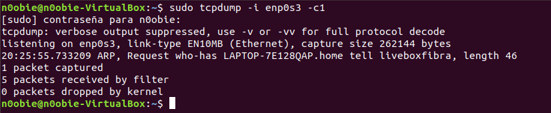
\includegraphics[width=14cm]{archivos/img/anexos/tcpdump_cli_edited.png}
    \caption{Interfaz CLI de Tcpdump}
    \label{tcpdumpCli}
\end{figure}

%%%%%%%%%%%%%%%%%%%%%%%%%%%%%%%%%%%%%%%%%%%%%%%%%%%%%%%%%%%%%%%%%%%%%%%%%%%%%%%%%%%%%%%%%%%%%%%%%%
